% Options for packages loaded elsewhere
\PassOptionsToPackage{unicode}{hyperref}
\PassOptionsToPackage{hyphens}{url}
%
\documentclass[
  12pt,
  spanish,
  10pt]{article}
\usepackage{lmodern}
\usepackage{amssymb,amsmath}
\usepackage{ifxetex,ifluatex}
\ifnum 0\ifxetex 1\fi\ifluatex 1\fi=0 % if pdftex
  \usepackage[T1]{fontenc}
  \usepackage[utf8]{inputenc}
  \usepackage{textcomp} % provide euro and other symbols
\else % if luatex or xetex
  \usepackage{unicode-math}
  \defaultfontfeatures{Scale=MatchLowercase}
  \defaultfontfeatures[\rmfamily]{Ligatures=TeX,Scale=1}
\fi
% Use upquote if available, for straight quotes in verbatim environments
\IfFileExists{upquote.sty}{\usepackage{upquote}}{}
\IfFileExists{microtype.sty}{% use microtype if available
  \usepackage[]{microtype}
  \UseMicrotypeSet[protrusion]{basicmath} % disable protrusion for tt fonts
}{}
\usepackage{xcolor}
\IfFileExists{xurl.sty}{\usepackage{xurl}}{} % add URL line breaks if available
\IfFileExists{bookmark.sty}{\usepackage{bookmark}}{\usepackage{hyperref}}
\hypersetup{
  pdftitle={Retenciones vs.~impuesto a las ganancias: impacto sobre el patrimonio de los productores},
  pdfauthor={Bolsa de Cereales},
  pdflang={es},
  hidelinks,
  pdfcreator={LaTeX via pandoc}}
\urlstyle{same} % disable monospaced font for URLs
\usepackage[margin=1in]{geometry}
\usepackage{longtable,booktabs}
% Correct order of tables after \paragraph or \subparagraph
\usepackage{etoolbox}
\makeatletter
\patchcmd\longtable{\par}{\if@noskipsec\mbox{}\fi\par}{}{}
\makeatother
% Allow footnotes in longtable head/foot
\IfFileExists{footnotehyper.sty}{\usepackage{footnotehyper}}{\usepackage{footnote}}
\makesavenoteenv{longtable}
\usepackage{graphicx}
\makeatletter
\def\maxwidth{\ifdim\Gin@nat@width>\linewidth\linewidth\else\Gin@nat@width\fi}
\def\maxheight{\ifdim\Gin@nat@height>\textheight\textheight\else\Gin@nat@height\fi}
\makeatother
% Scale images if necessary, so that they will not overflow the page
% margins by default, and it is still possible to overwrite the defaults
% using explicit options in \includegraphics[width, height, ...]{}
\setkeys{Gin}{width=\maxwidth,height=\maxheight,keepaspectratio}
% Set default figure placement to htbp
\makeatletter
\def\fps@figure{htbp}
\makeatother
\setlength{\emergencystretch}{3em} % prevent overfull lines
\providecommand{\tightlist}{%
  \setlength{\itemsep}{0pt}\setlength{\parskip}{0pt}}
\setcounter{secnumdepth}{5}

\ifxetex
  % Load polyglossia as late as possible: uses bidi with RTL langages (e.g. Hebrew, Arabic)
  \usepackage{polyglossia}
  \setmainlanguage[]{spanish}
\else
  \usepackage[shorthands=off,main=spanish]{babel}
\fi
\ifluatex
  \usepackage{selnolig}  % disable illegal ligatures
\fi

\title{Retenciones vs.~impuesto a las ganancias: impacto sobre el
patrimonio de los productores}
\author{Bolsa de Cereales}
\date{16 de noviembre de 2020}

\begin{document}
\maketitle

{
\setcounter{tocdepth}{1}
\tableofcontents
}
\hypertarget{introducciuxf3n}{%
\section{Introducción}\label{introducciuxf3n}}

Existe consenso sobre el impacto negativo de las retenciones sobre las
actividades agropecuarias: al reducir la rentabilidad desincentiva
inversión en tecnología, el uso de fertilizantes y reduce la superficie
sembrada. El argumento principal para aplicar retenciones es la
capacidad recaudatoria del impuesto: en la campaña 19/20 se recaudará en
torno a USD 5.600 millones (complejo soja).

Una de las características que hace que las retenciones sean un mal
impuesto es su carácter pro-cíclico: cuando los productores tienen una
campaña mala (buena) las retenciones representan una proporción mayor
(menor) de su ingreso. En ese marco, creemos que incrementar el impuesto
a las ganancias, que no es procíclico, y reducir los derechos de
exportación puede resultar una respuesta más inteligente para promover
la producción sin desfinanciar al fisco.

En ese sentido. el objetivo de este trabajo es mostrar, aplicando
simulaciones, como impactan un incremento de las retenciones y del
impuesto a las ganancias sobre la rentabilidad y el patrimonio de los
productores y la recaudación nacional. Para ello se elaboraron tres
escenarios para los cuales se analiza la dinámica de las variables
mencionadas. Los escenarios simulados son los siguientes:

\begin{itemize}
\tightlist
\item
  Escenario 1 \textbf{`Situación Actual'}: 33\% de alícuota de derechos
  de exportación (DEX) a soja y 30\% de alícuota de ganancias.
\item
  Escenario 2 \textbf{`Aumento de Retenciones, manteniendo la alícuota
  de ganancias'}: 35\% de alícuota DEX y 30\% de alícuota de ganancias.
\item
  Escenario 3 \textbf{`Aumento de Ganancias con baja de retenciones'}:
  28\% de alícuota DEX y 35\% de alícuota de impuesto a las ganancias.
\end{itemize}

Los principales resultados del trabajo son: (i) que con los niveles
actuales de DEX y alicuota de ganancias puede puede llevar a un brusco
deterioro de la situación patrimonial de los productores en el mediano
plazo y (ii) que el impuesto a las ganancias permite recaudar un monto
similar sin afectar significativamente la sustentabilidad económica.

El resto del documento se estrucutra de la siguiente manera en la
sección 2 se describen las variables aleatorias a partir de las cuales
se elaboran los escenarios. En la sección 3 se describen los resultados
de las simulaciones. En la sección 4 se comparan los resultados de los
distintos escenarios. Por último en la sección 5 se resumen las
principales conclusiones.

\hypertarget{variables-estocuxe1sticas}{%
\section{Variables estocásticas:}\label{variables-estocuxe1sticas}}

Existen dos variables incontrolables para el productor con fuerte
incidencia en la rentabilidad de las explotaciones agrícolas: el clima y
los precios.

\hypertarget{rendimientos}{%
\subsection{Rendimientos}\label{rendimientos}}

Como el clima afecta directamente los rendimientos, en nuestras
simulaciones asumimos que los rendimientos presentan una distribución
normal con media 33 quintales y desvío de 9 quintales.

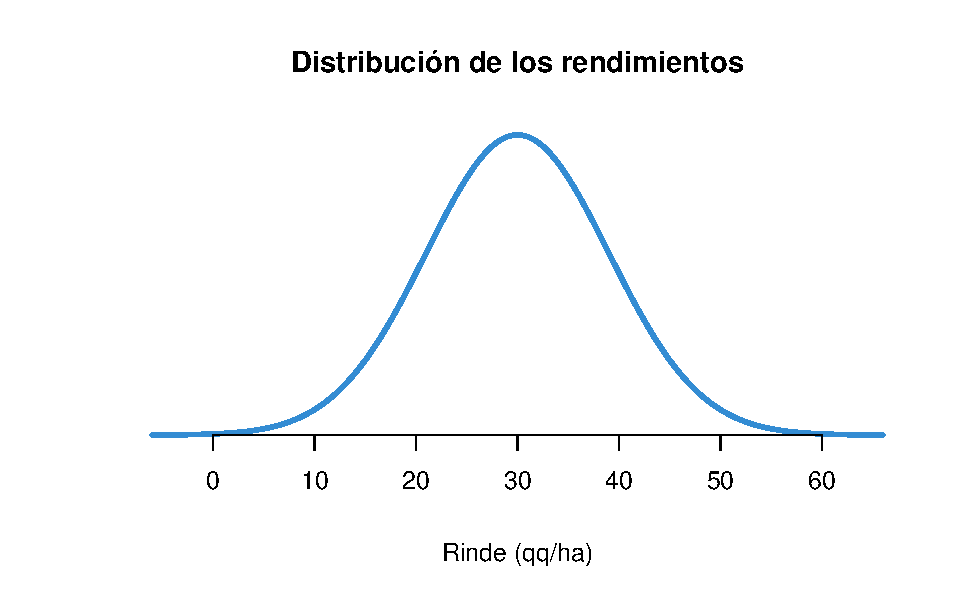
\includegraphics{simulacion_retenciones_bagging_files/figure-latex/unnamed-chunk-2-1.pdf}

\hypertarget{precios}{%
\subsection{Precios}\label{precios}}

En el mismo sentido, los precios se forman en los mercados
internacionales y su dinámica es exógena a lo que suceda en nuestro
país. En nuestras simulaciones se asume que los precios del poroto de
soja tienen una distribución normal con media USD 330 por tonelada y un
desvío de USD 40 por tonelada. De esta forma, el 95\% de los precios se
ubicaran en el rango 250 - 410 USD/tn.

\begin{center}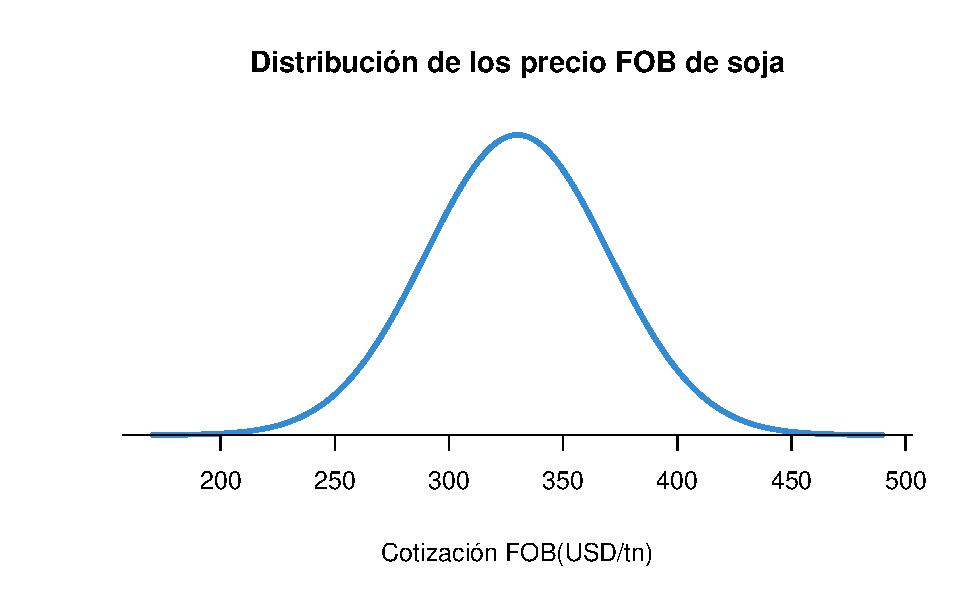
\includegraphics{simulacion_retenciones_bagging_files/figure-latex/unnamed-chunk-4-1} \end{center}

\hypertarget{simulando-las-campauxf1as}{%
\section{Simulando las campañas}\label{simulando-las-campauxf1as}}

Se asume que los productores tiene un patrimonio inicial que les permite
costear tres campañas.

Cada campaña los productores invierten y obtienen un rendimiento
aleatorio que sigue la distribución descripta anteriormente. Venden su
producción a un precio que también es aleatorio y que sigue la
distribución descripta anteriormente.

Los ingresos brutos (rendimiento*precio) están afectados por los
impuestos. En el caso de las retenciones, a través de un precio FAS más
bajo, en el caso de ganancias se le descuenta el impuesto solo si
registra un resultado neto (diferencia entre ingreso bruto y costos de
producción) positivo.

De esta manera, cada campaña el patrimonio del productor puede
incrementarse o reducirse. Se asume que el productor participa en las
campañas siempre y cuando tengo un patrimonio neto positivo.

A través de esta simulación podemos ver que estructura impositiva es más
efectiva para recaudar más afectando menos la sustentabilidad económica
de los productores.

\hypertarget{simulaciuxf3n-escenario-1}{%
\subsection{Simulación escenario 1:}\label{simulaciuxf3n-escenario-1}}

Parámetros escenario 1:

\begin{itemize}
\tightlist
\item
  33\% de Alícuota de retención y 30\% de impuesto a las ganancias.
\end{itemize}

\hypertarget{resultados-escenario-1}{%
\subsection{Resultados escenario 1}\label{resultados-escenario-1}}

\begin{longtable}[]{@{}lr@{}}
\toprule
Variable & Valor\tabularnewline
\midrule
\endhead
Escenario & 1.00\tabularnewline
Alícuota DEX & 0.33\tabularnewline
Tasa Imp. Gananacias & 0.30\tabularnewline
Nº de períodos hasta quebranto & 999.00\tabularnewline
Recaudación total & 235290.00\tabularnewline
Proporción de campañas con resultado positivo & 81.80\tabularnewline
Resultado económico medio & 32.35\tabularnewline
\bottomrule
\end{longtable}

Las salidas del escenario 1 se interpretan de la siguiente manera:

\begin{itemize}
\tightlist
\item
  el productor nunca pierde todo su patrimonio (se corren en total 1000
  campañas)
\item
  el gobierno recauda, a lo largo de las 1000 campañas, \textbf{USD 230
  644} por hectárea
\item
  El productor \textbf{tiene un resultado negativo el 56.9\% de las
  campañas}
\item
  En promedio el productor \textbf{gana 23.8 dólares por hectárea cada
  campaña}
\end{itemize}

\hypertarget{simulaciuxf3n-escenario-2}{%
\subsection{Simulación escenario 2}\label{simulaciuxf3n-escenario-2}}

Parámetros Escenario 2:

\begin{itemize}
\tightlist
\item
  35\% de Alícuota de retención y 30\% de impuesto a las ganancias.
\end{itemize}

\hypertarget{resultados-escenario-2}{%
\subsection{Resultados escenario 2}\label{resultados-escenario-2}}

\begin{longtable}[]{@{}lr@{}}
\toprule
Variable & Valor\tabularnewline
\midrule
\endhead
Escenario & 2.00\tabularnewline
Alícuota DEX & 0.35\tabularnewline
Tasa Imp. Gananacias & 0.30\tabularnewline
Nº de períodos hasta quebranto & 999.00\tabularnewline
Recaudación total & 236974.00\tabularnewline
Proporción de campañas con resultado positivo & 71.60\tabularnewline
Resultado económico medio & 21.35\tabularnewline
\bottomrule
\end{longtable}

Las salidas del \textbf{escenario 2} se interpretan de la siguiente
manera:

\begin{itemize}
\tightlist
\item
  el productor pierde todo su patrimonio al cabo de \textbf{113
  campañas}
\item
  el gobierno recauda, a lo largo de las 60 campañas, USD 24137 por
  hectárea
\item
  El productor tiene un \textbf{resultado positivo solo el 50.4\%} de
  las campañas
\item
  En promedio el productor \textbf{pierde 8.55 dólares por hectarea cada
  campaña}
\end{itemize}

\hypertarget{simulaciuxf3n-escenario-3}{%
\subsection{Simulación escenario 3}\label{simulaciuxf3n-escenario-3}}

Parámetros escenario 3:

\begin{itemize}
\tightlist
\item
  28\% de alícuota de retención y 35\% de impuesto a las ganancias.
\end{itemize}

\hypertarget{resultados-escenario-3}{%
\subsection{Resultados escenario 3}\label{resultados-escenario-3}}

\begin{longtable}[]{@{}lr@{}}
\toprule
Variable & Valor\tabularnewline
\midrule
\endhead
Escenario & 3.00\tabularnewline
Alícuota DEX & 0.28\tabularnewline
Tasa Imp. Gananacias & 0.35\tabularnewline
Nº de períodos hasta quebranto & 999.00\tabularnewline
Recaudación total & 235598.00\tabularnewline
Proporción de campañas con resultado positivo & 94.70\tabularnewline
Resultado económico medio & 52.12\tabularnewline
\bottomrule
\end{longtable}

Las salidas del \textbf{escenario 3} se interpretan de la siguiente
manera:

\begin{itemize}
\tightlist
\item
  el productor nunca pierde todo su patrimonio (se corren en total 1000
  campañas)
\item
  el gobierno recauda, a lo largo de las 1000 campañas, USD 230 770 por
  hectárea
\item
  El productor tiene un \textbf{resultado positivo el 62.8\%} de las
  campañas
\item
  En promedio el productor \textbf{gana 43.29 dólares por hectarea cada
  campaña}
\end{itemize}

\hypertarget{resultados-conjuntos}{%
\section{Resultados conjuntos}\label{resultados-conjuntos}}

\hypertarget{evoluciuxf3n-del-patrimonio-neto-del-productor}{%
\subsection{Evolución del patrimonio neto del
productor}\label{evoluciuxf3n-del-patrimonio-neto-del-productor}}

En el escenario de mayores retenciones el patrimonio neto (PN) del
productor se vuelve negativo al cabo de 14 campañas. Notablemente más
rápido que en los escenarios alternativos, en los que el PN se mantiene
estable.

\begin{center}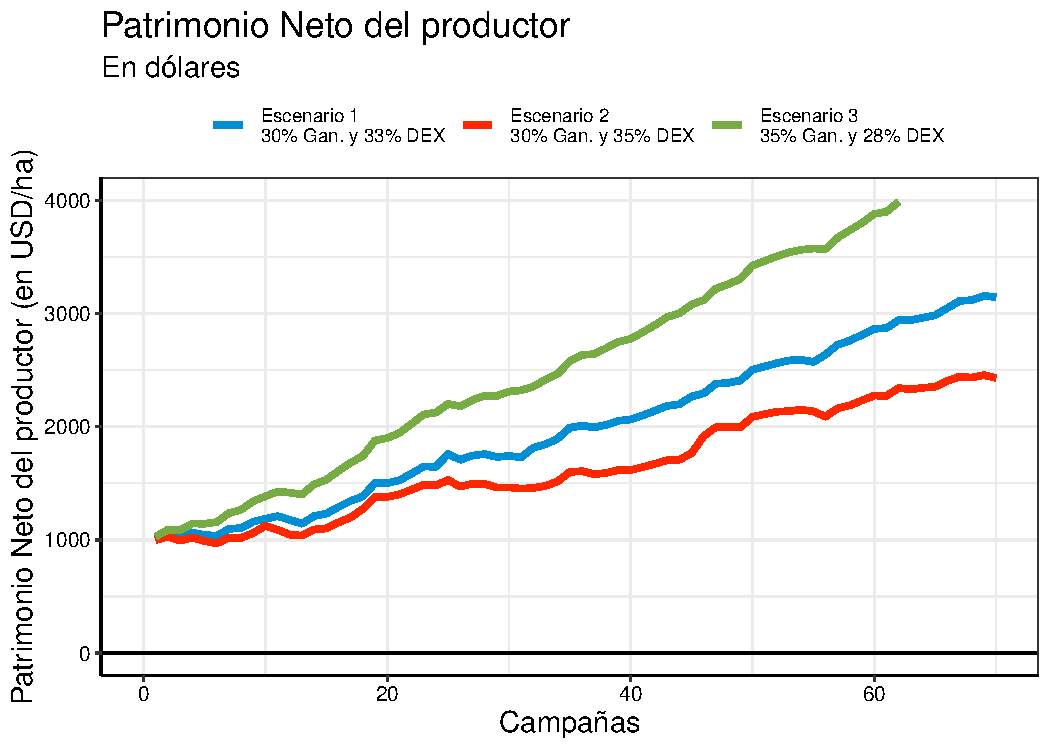
\includegraphics{simulacion_retenciones_bagging_files/figure-latex/unnamed-chunk-16-1} \end{center}

\hypertarget{resultado-econuxf3mico}{%
\subsection{Resultado Económico}\label{resultado-econuxf3mico}}

La distribución de los resultados económicos difiere en los distintos
escenarios siendo notoriamente peor en el caso del aumento de
retenciones.

Se entiende como resultado económico como ingreso neto de costos de
producción y pago de impuestos (ganancias).

Sobre este punto se destaca que el escenarios 1 y 2 (mayores
retenciones) presentan una distribución bimodal muy acentuada. Esto
significa que los resutlados económicos en ese escenario son estan mas
polarizados. Esto se debe al caracter prociclico de las retenciones.

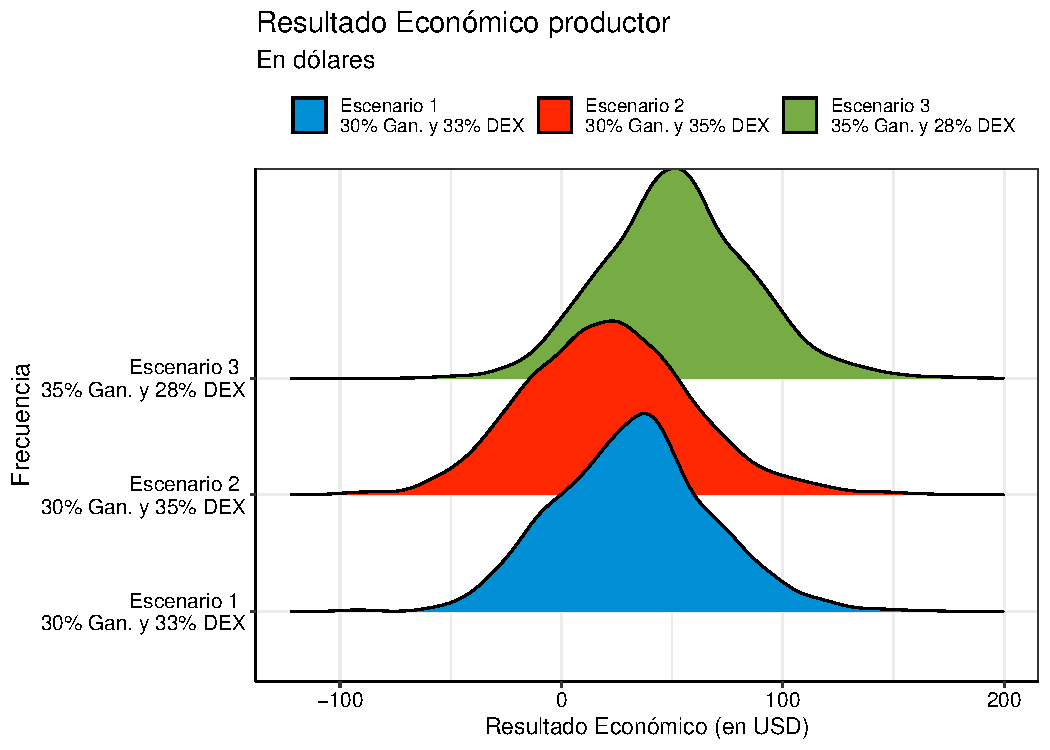
\includegraphics{simulacion_retenciones_bagging_files/figure-latex/unnamed-chunk-18-1.pdf}

\hypertarget{proporciuxf3n-de-campauxf1as-con-resultado-econuxf3mico-positivo}{%
\subsection{Proporción de campañas con resultado económico
positivo}\label{proporciuxf3n-de-campauxf1as-con-resultado-econuxf3mico-positivo}}

En el gráfico siguiente se presenta la proporción de campañas con
resultado económico positivo como proporción del total de campañas. El
gráfico muestra que el escenario de mayores retenciones hace que cerca
del 50\% de las campañas arrojen pérdidas, mientras que en el caso de
mayores impuestos a las ganancias la proporción de campañas con pérdidas
de 37\%.

En este sentido, se puede destacar que incrementar el impuesto a las
ganancias permite incrementar la recaudación sin poner en riesgo la
sustentabilidad económica de los productores.

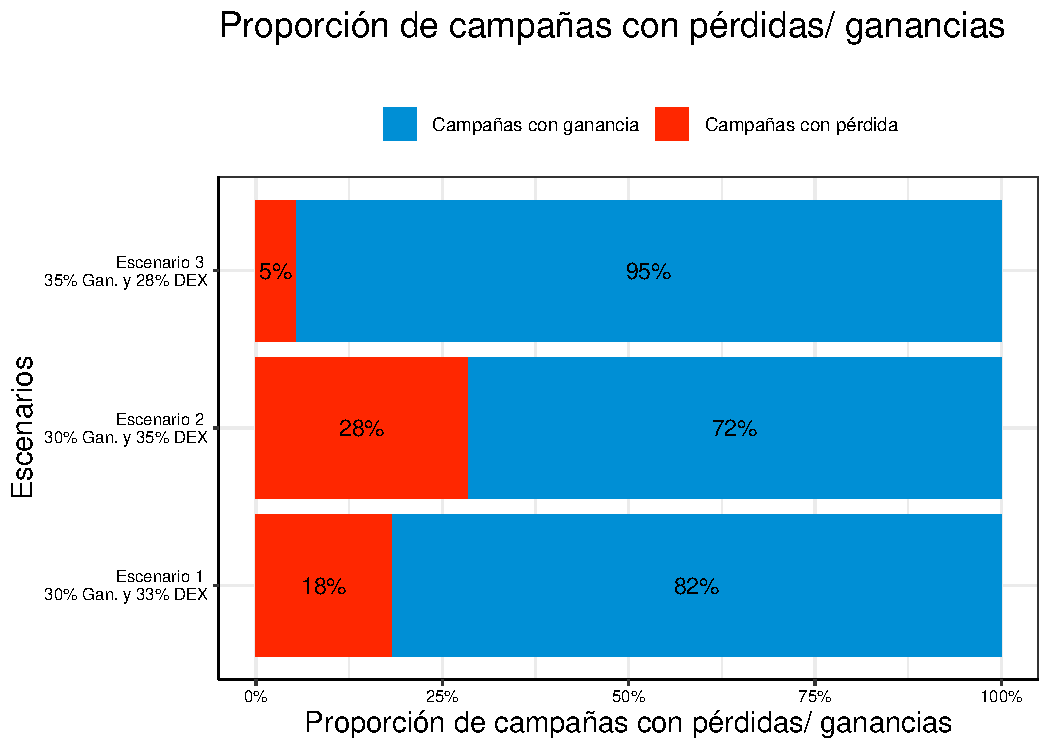
\includegraphics{simulacion_retenciones_bagging_files/figure-latex/unnamed-chunk-19-1.pdf}

\hypertarget{conclusiones}{%
\section{Conclusiones}\label{conclusiones}}

\begin{itemize}
\item
  Las retenciones son procíclicas y afectan más a los productores en los
  años con mal clima o malos precios.
\item
  La situación actual de alicuotas de 33\% puede puede llevar a un
  brusco deterioro de la situación patrimonial de los productores en
  contextos de sequía o deterioro de los precios internacionales.
\item
  El impuesto a las ganancias permite recaudar un monto similar sin
  afectar significativamente la sustentabilidad económica.
\end{itemize}

\end{document}
